\begin{figure}[t]\centering
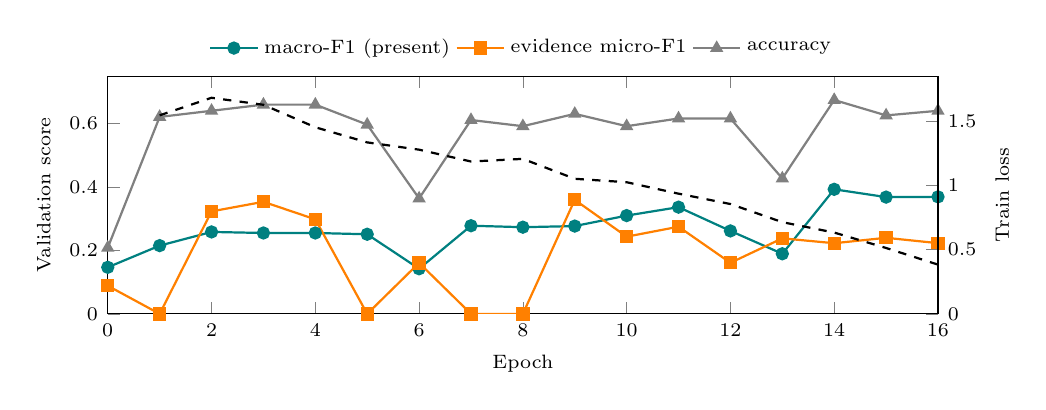
\begin{tikzpicture}\begin{axis}[width=\columnwidth,height=4.6cm,xlabel={Epoch},ylabel={Validation score},ymin=0,ymax=0.75,
legend style={font=\scriptsize,at={(0.5,1.03)},anchor=south,legend columns=3,draw=none},tick label style={font=\scriptsize},label style={font=\scriptsize},
axis y line*=left,xmin=0,xmax=16]
\addplot[thick,mark=*,color=teal] coordinates {(0,0.1469) (1,0.2153) (2,0.2585) (3,0.2552) (4,0.2552) (5,0.2512) (6,0.1423) (7,0.2781) (8,0.2735) (9,0.2770) (10,0.3101) (11,0.3367) (12,0.2617) (13,0.1896) (14,0.3930) (15,0.3684) (16,0.3692)};\addlegendentry{macro-F1 (present)}
\addplot[thick,mark=square*,color=orange] coordinates {(0,0.0887) (1,0.0000) (2,0.3234) (3,0.3536) (4,0.2983) (5,0.0000) (6,0.1609) (7,0.0000) (8,0.0000) (9,0.3598) (10,0.2436) (11,0.2750) (12,0.1611) (13,0.2383) (14,0.2229) (15,0.2400) (16,0.2231)};\addlegendentry{evidence micro-F1}
\addplot[thick,mark=triangle*,color=gray] coordinates {(0,0.2087) (1,0.6214) (2,0.6408) (3,0.6602) (4,0.6602) (5,0.5971) (6,0.3641) (7,0.6117) (8,0.5922) (9,0.6311) (10,0.5922) (11,0.6165) (12,0.6165) (13,0.4272) (14,0.6748) (15,0.6262) (16,0.6408)};\addlegendentry{accuracy}
\end{axis}
\begin{axis}[width=\columnwidth,height=4.6cm,axis y line*=right,axis x line=none,ylabel={Train loss},ymin=0,xmin=0,xmax=16,
tick label style={font=\scriptsize},label style={font=\scriptsize}]
\addplot[dashed,thick,color=black] coordinates {(1,1.5429) (2,1.6790) (3,1.6247) (4,1.4500) (5,1.3324) (6,1.2759) (7,1.1839) (8,1.2044) (9,1.0496) (10,1.0229) (11,0.9339) (12,0.8535) (13,0.7125) (14,0.6317) (15,0.5119) (16,0.3827)};
\end{axis}\end{tikzpicture}
\caption{Validation metrics per epoch (solid, left axis; epoch 0 is the unadapted base) and mean training loss (dashed, right axis). The checkpoint with the best selection score (epoch 9) was frozen.}\label{fig:train}\end{figure}

\begin{figure}[t]\centering
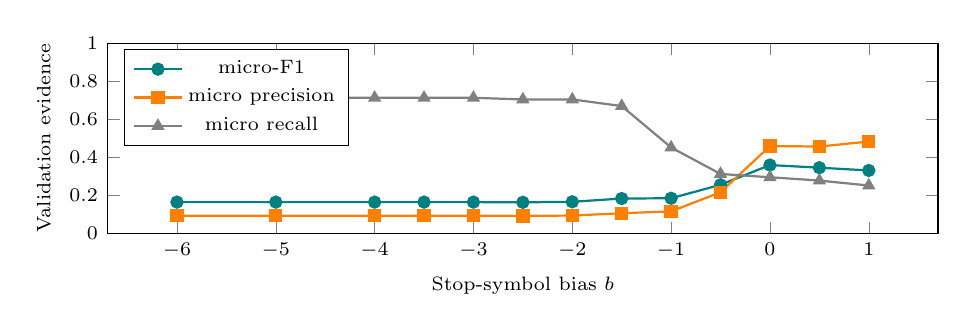
\begin{tikzpicture}\begin{axis}[width=\columnwidth,height=4cm,xlabel={Stop-symbol bias $b$},ylabel={Validation evidence},ymin=0,ymax=1,
legend style={font=\scriptsize,at={(0.02,0.97)},anchor=north west},tick label style={font=\scriptsize},label style={font=\scriptsize}]
\addplot[thick,mark=*,color=teal] coordinates {(1,0.3314) (0.5,0.3459) (0,0.3598) (-0.5,0.2562) (-1,0.1854) (-1.5,0.1840) (-2,0.1668) (-2.5,0.1641) (-3,0.1652) (-3.5,0.1652) (-4,0.1652) (-5,0.1652) (-6,0.1652)};\addlegendentry{micro-F1}
\addplot[thick,mark=square*,color=orange] coordinates {(1,0.4833) (0.5,0.4571) (0,0.4595) (-0.5,0.2169) (-1,0.1166) (-1.5,0.1066) (-2,0.0946) (-2.5,0.0929) (-3,0.0934) (-3.5,0.0934) (-4,0.0934) (-5,0.0934) (-6,0.0934)};\addlegendentry{micro precision}
\addplot[thick,mark=triangle*,color=gray] coordinates {(1,0.2522) (0.5,0.2783) (0,0.2957) (-0.5,0.3130) (-1,0.4522) (-1.5,0.6696) (-2,0.7043) (-2.5,0.7043) (-3,0.7130) (-3.5,0.7130) (-4,0.7130) (-5,0.7130) (-6,0.7130)};\addlegendentry{micro recall}
\end{axis}\end{tikzpicture}
\caption{Validation-only sweep of the additive stop-symbol bias. Lower $b$ makes the decoder cite more sentences, trading precision for recall; $b=0$ maximises micro-F1 and was frozen before testing.}\label{fig:cal}\end{figure}

\begin{table}[t]\centering\caption{All adaptation runs, validation split only (best epoch by the selection score)}\label{tab:runs}\footnotesize
\begin{tabular}{lrrrrrr}
\hline
Configuration & Ep. & Best & Acc. & MF1$_p$ & Ev.F1 & Sel.\\\hline
14M, unw. (1st subm.), 2e-4, 4\,ep & 4 & 4 & 0.621 & 0.219 & 0.000 & 0.109\\
14M, bal.\,$p{=}$0.5, ev+stop $\times$3, 3e-4 & 3 & 1 & 0.621 & 0.215 & 0.000 & 0.108\\
14M, unw., ev+stop $\times$3, 3e-4 & 3 & 1 & 0.621 & 0.215 & 0.000 & 0.108\\
14M, bal.\,$p{=}$0.5, ev $\times$5, 3e-4 & 6 & 3 & 0.617 & 0.213 & 0.017 & 0.115\\
14M, bal.\,$p{=}$0.5, ev $\times$5, 1e-3 & 6 & 5 & 0.626 & 0.218 & 0.000 & 0.109\\
70M, bal.\,$p{=}$1, ev $\times$5, 2e-4, 10\,ep & 10 & 10 & 0.650 & 0.328 & 0.250 & 0.289\\
70M, bal.\,$p{=}$1, ev $\times$5, 2e-4, 16\,ep & 16 & 9 & 0.631 & 0.277 & 0.360 & 0.318\\
\hline\end{tabular}
\\[2pt]\parbox{0.98\linewidth}{\scriptsize ``ev+stop'' runs used an early weighting bug that also up-weighted the stop symbol; 14M runs were stopped early once collapse was evident. The last row is the frozen model.}
\end{table}

\begin{table}[t]\centering\caption{Latent signal on validation from teacher-forced logits (ROC-AUC; 0.5 = chance)}\label{tab:diag}\footnotesize
\begin{tabular}{lrrrr}
\hline
Model & Mean label & Included & Excl. N/A & Evidence\\\hline
Pythia-14M base & 0.56 & 0.61 & 0.29 & 0.46\\
Pythia-14M 1st subm. & 0.46 & 0.52 & 0.44 & 0.66\\
Pythia-70M base & 0.55 & 0.56 & 0.48 & 0.51\\
Pythia-70M final & 0.53 & 0.71 & 0.74 & 0.69\\
\hline\end{tabular}
\end{table}

\begin{table}[t]\centering\caption{Fine-tuning configuration (Pythia-70M target)}\label{tab:hparams}\footnotesize
\begin{tabular}{ll}
\hline
Setting & Value\\\hline
Trainable / total parameters & 18,970,112 / 44,725,760\\
Frozen & input embedding (25.8M)\\
Objective & answer-only teacher-forced CE\\
Label weights & balanced, power 1\\
Evidence-ID weight & 5 (stop symbol 1)\\
Optimiser & AdamW, wd 0.01, clip 1.0\\
Learning rate & 0.0002, 6\% warm-up, linear decay\\
Batch & 1 record, accumulate 4\\
Epochs / selected & 16 / 9\\
Precision / threads / seed & FP32 / 6 CPU / 42\\
\hline\end{tabular}
\end{table}

\begin{table*}[t]\centering\caption{Paired before/after comparison on identical validation and held-out test rows (constrained greedy decoding)}\label{tab:scores}\footnotesize
\begin{tabular}{llcccccccccc}
\hline
Split & System & Acc. & MF1$_6$ & MF1$_p$ & Acc$_{inc}$ & Acc$_{exc}$ & Ev.P & Ev.R & Ev.F1$_\mu$ & Ev.F1$_M$ & Ev.F1$_M^{+}$\\\hline
Validation & Majority & 0.621 & 0.215 & 0.215 & 0.409 & 0.721 & 0.000 & 0.000 & 0.000 & 0.563 & 0.000\\
Validation & Maj.+lead sent. & 0.621 & 0.215 & 0.215 & 0.409 & 0.721 & 0.204 & 0.365 & 0.262 & 0.178 & 0.407\\
Validation & 1st subm. 14M & 0.621 & 0.219 & 0.219 & 0.409 & 0.721 & 0.000 & 0.000 & 0.000 & 0.563 & 0.000\\
Validation & Base 70M & 0.209 & 0.147 & 0.147 & 0.530 & 0.057 & 0.102 & 0.078 & 0.089 & 0.468 & 0.071\\
Validation & Adapted (final) & 0.631 & 0.277 & 0.277 & 0.409 & 0.736 & 0.459 & 0.296 & 0.360 & 0.602 & 0.334\\
Test & Majority & 0.626 & 0.226 & 0.272 & 0.507 & 0.695 & 0.000 & 0.000 & 0.000 & 0.704 & 0.000\\
Test & Maj.+lead sent. & 0.626 & 0.226 & 0.272 & 0.507 & 0.695 & 0.184 & 0.404 & 0.253 & 0.150 & 0.508\\
Test & 1st subm. 14M & 0.612 & 0.222 & 0.266 & 0.507 & 0.672 & 0.000 & 0.000 & 0.000 & 0.704 & 0.000\\
Test & Base 70M & 0.194 & 0.144 & 0.173 & 0.360 & 0.099 & 0.099 & 0.149 & 0.119 & 0.549 & 0.083\\
Test & Adapted (final) & 0.631 & 0.279 & 0.334 & 0.507 & 0.702 & 0.315 & 0.245 & 0.275 & 0.635 & 0.340\\
\hline\end{tabular}
\\[2pt]\parbox{0.95\linewidth}{\scriptsize MF1$_6$: macro-F1 over all six labels (zero-support classes count as 0); MF1$_p$: over labels present in the gold set. Ev.\ = evidence sentence retrieval; $\mu$ micro (pooled), $M$ per-record macro where two empty sets score 1, $M^{+}$ macro over records with non-empty gold evidence only. Majority = type-conditioned training majority label without evidence; Maj.+lead sent.\ adds the first note sentence as evidence; 1st subm.\ = our original Pythia-14M submission re-scored with these metrics.}
\end{table*}

\begin{table}[t]\centering\caption{Adapted model, held-out test, inclusion criteria ($n=75$): per-class scores and confusion matrix (rows gold, columns predicted)}\label{tab:cls_inclusion}\footnotesize
\begin{tabular}{lrccc|rrrr}
\hline
Gold & n & P & R & F1 & Incl. & Not incl. & NEI & N/A\\\hline
Incl. & 27 & 0.000 & 0.000 & 0.000 & 0 & 0 & 27 & 0\\
Not incl. & 7 & 0.000 & 0.000 & 0.000 & 0 & 0 & 7 & 0\\
NEI & 38 & 0.507 & 1.000 & 0.673 & 0 & 0 & 38 & 0\\
N/A & 3 & 0.000 & 0.000 & 0.000 & 0 & 0 & 3 & 0\\
\hline\end{tabular}
\end{table}

\begin{table}[t]\centering\caption{Adapted model, held-out test, exclusion criteria ($n=131$): per-class scores and confusion matrix (rows gold, columns predicted)}\label{tab:cls_exclusion}\footnotesize
\begin{tabular}{lrccc|rrrr}
\hline
Gold & n & P & R & F1 & Excl. & Not excl. & NEI & N/A\\\hline
Excl. & 0 & 0.000 & 0.000 & 0.000 & 0 & 0 & 0 & 0\\
Not excl. & 91 & 0.706 & 0.978 & 0.820 & 0 & 89 & 1 & 1\\
NEI & 28 & 0.000 & 0.000 & 0.000 & 0 & 28 & 0 & 0\\
N/A & 12 & 0.750 & 0.250 & 0.375 & 0 & 9 & 0 & 3\\
\hline\end{tabular}
\end{table}

\begin{table}[t]\centering\caption{Held-out test per-label F1 and prediction counts before (base) and after adaptation}\label{tab:classes}\footnotesize
\begin{tabular}{lrcccc}
\hline
Label & Support & F1 base & F1 adapt. & \#pred base & \#pred adapt.\\\hline
Incl. & 27 & 0.529 & 0.000 & 75 & 0\\
Not incl. & 7 & 0.000 & 0.000 & 0 & 0\\
Excl. & 0 & 0.000 & 0.000 & 87 & 0\\
Not excl. & 91 & 0.000 & 0.820 & 0 & 126\\
NEI & 66 & 0.224 & 0.535 & 41 & 76\\
N/A & 15 & 0.111 & 0.316 & 3 & 4\\
\hline\end{tabular}
\end{table}

\begin{table*}[t]\centering\caption{Test difference of the adapted model with patient-level 95\% bootstrap intervals (5000 resamples of the 8 test patients)}\label{tab:ci}\footnotesize
\begin{tabular}{lccc}
\hline
Adapted & $\Delta$Acc. & $\Delta$MF1$_p$ & $\Delta$Ev.F1$_\mu$\\\hline
vs.\ majority & +0.005 [-0.012, +0.020] & +0.062 [+0.000, +0.130] & +0.275 [+0.181, +0.368]\\
vs.\ maj.+lead & +0.005 [-0.012, +0.020] & +0.062 [+0.000, +0.130] & +0.022 [-0.063, +0.106]\\
vs.\ base 70M & +0.437 [+0.163, +0.646] & +0.161 [+0.013, +0.315] & +0.156 [+0.056, +0.326]\\
\hline\end{tabular}
\\[2pt]\parbox{0.95\linewidth}{\scriptsize Exact McNemar test on label correctness, adapted vs.\ majority: 3 vs.\ 2 discordant criteria, $p=1.00$.}
\end{table*}

\begin{table*}[t]\centering\caption{Controlled greedy decoding on the adapted 70M target (stop suppressed; warm-up + median of 5; CPU, 2 threads)}\label{tab:runtime}\footnotesize
\begin{tabular}{llrrrrrrrrc}
\hline
In/out & Path & Prefill & Decode & Total ms & Tok/s & $\times$unc. & RSS MiB & KV KiB & Acc./prop. & Equal\\\hline
32/8 & uncached & 21.1 & 169.7 & 190.8 & 41.9 & 1.00 & 643 & -- & -- & yes\\
32/8 & cached & 22.2 & 43.2 & 65.3 & 122.4 & 2.92 & 643 & 960 & -- & yes\\
32/8 & speculative (early-exit) & -- & -- & 161.5 & 49.5 & 1.18 & 618 & -- & 0/26 & yes\\
32/8 & speculative (14M) & -- & -- & 77.9 & 102.7 & 2.52 & 618 & -- & 7/7 & yes\\
256/32 & uncached & 82.3 & 2791.5 & 2873.8 & 11.1 & 1.00 & 678 & -- & -- & yes\\
256/32 & cached & 90.2 & 218.1 & 308.2 & 103.8 & 9.32 & 677 & 6912 & -- & yes\\
256/32 & speculative (early-exit) & -- & -- & 336.1 & 95.2 & 8.55 & 657 & -- & 22/40 & yes\\
256/32 & speculative (14M) & -- & -- & 704.0 & 45.5 & 4.03 & 664 & -- & 7/98 & yes\\
1024/64 & uncached & 387.5 & 24756.7 & 25144.2 & 2.5 & 1.00 & 810 & -- & -- & yes\\
1024/64 & cached & 395.2 & 665.4 & 1060.6 & 60.3 & 23.71 & 806 & 26112 & -- & yes\\
1024/64 & speculative (early-exit) & -- & -- & 1124.9 & 56.9 & 22.35 & 799 & -- & 45/74 & yes\\
1024/64 & speculative (14M) & -- & -- & 2143.7 & 29.9 & 11.85 & 785 & -- & 12/205 & yes\\
\hline\end{tabular}
\\[2pt]\parbox{0.95\linewidth}{\scriptsize Prefill and decode are timed separately for the two non-speculative paths; speculative time is end-to-end (both prefills included). KV KiB is the analytic FP32 cache size at the end of generation. RSS is sampled process memory (interpreter, all models) and can miss short peaks. Equal: token sequence identical to the uncached reference.}
\end{table*}

\begin{table}[t]\centering\caption{Real screening outputs (grammar and stop enabled) on 24 validation criteria: mean latency per criterion}\label{tab:screening}\footnotesize
\begin{tabular}{lrrrrrr}
\hline
Path & n & Mean ms & Out tok. & Accepted & Rate & Equal\\\hline
uncached & 24 & 184.5 & 2.33 & -- & -- & 24/24\\
cached & 24 & 88.4 & 2.33 & -- & -- & 24/24\\
speculative (early-exit) & 24 & 131.7 & 2.33 & 24/104 & 23\% & 24/24\\
speculative (14M) & 24 & 106.0 & 2.33 & 55/57 & 96\% & 24/24\\
\hline\end{tabular}
\end{table}

\begin{table*}[t]\centering\caption{Attention kernels vs.\ an FP64 SDPA ground truth (4 heads, $d_h=32$, FP32, median of 5)}\label{tab:attention}\footnotesize
\begin{tabular}{lccrrrrrrrr}
\hline
$L_q\times L_k$ & C & Blk & Ref max & Tiled max & Tiled mean & Ref ms & Tiled ms & SDPA ms & Full KiB & Tile KiB\\\hline
17$\times$17 & y & 32 & 5.4e-07 & 5.4e-07 & 4.1e-08 & 0.22 & 0.39 & 0.07 & 5 & 5\\
17$\times$17 & n & 32 & 5.4e-07 & 5.4e-07 & 4.5e-08 & 0.15 & 0.25 & 0.06 & 5 & 5\\
65$\times$65 & y & 32 & 4.7e-07 & 5.0e-07 & 3.5e-08 & 0.31 & 1.43 & 0.13 & 66 & 16\\
65$\times$65 & n & 32 & 3.8e-07 & 3.8e-07 & 3.1e-08 & 0.20 & 1.43 & 0.09 & 66 & 16\\
256$\times$256 & y & 32 & 6.1e-07 & 6.1e-07 & 2.6e-08 & 1.45 & 7.35 & 0.59 & 1024 & 16\\
256$\times$256 & n & 32 & 3.5e-07 & 2.6e-07 & 1.8e-08 & 0.52 & 10.09 & 0.47 & 1024 & 16\\
512$\times$512 & y & 32 & 6.7e-07 & 6.1e-07 & 2.1e-08 & 5.74 & 25.09 & 2.05 & 4096 & 16\\
512$\times$512 & n & 32 & 5.4e-07 & 2.6e-07 & 1.4e-08 & 2.39 & 36.24 & 1.31 & 4096 & 16\\
1$\times$300 & y & 32 & 7.0e-08 & 5.4e-08 & 1.4e-08 & 0.18 & 1.54 & 0.06 & 5 & 0\\
1$\times$300 & n & 32 & 7.0e-08 & 5.4e-08 & 1.4e-08 & 0.13 & 1.26 & 0.06 & 5 & 0\\
40$\times$300 & y & 32 & 2.4e-07 & 3.2e-07 & 1.9e-08 & 0.35 & 3.46 & 0.21 & 188 & 16\\
40$\times$300 & n & 32 & 2.8e-07 & 2.8e-07 & 1.9e-08 & 0.24 & 2.71 & 0.16 & 188 & 16\\
256$\times$256 & y & 8 & 6.1e-07 & 5.6e-07 & 2.6e-08 & 1.36 & 74.73 & 0.52 & 1024 & 1\\
256$\times$256 & y & 16 & 6.1e-07 & 5.4e-07 & 2.5e-08 & 1.44 & 20.73 & 0.55 & 1024 & 4\\
256$\times$256 & y & 64 & 6.1e-07 & 6.1e-07 & 2.7e-08 & 1.41 & 2.66 & 0.55 & 1024 & 64\\
256$\times$256 & y & 128 & 6.1e-07 & 6.1e-07 & 3.0e-08 & 1.27 & 1.40 & 0.57 & 1024 & 256\\
\hline\end{tabular}
\\[2pt]\parbox{0.95\linewidth}{\scriptsize Errors are maximum/mean absolute differences from FP64 \texttt{scaled\_dot\_product\_attention}. Full/Tile KiB: size of the score matrix materialised by the reference versus the largest single tile of the online-softmax kernel. Rectangular shapes ($L_q<L_k$) model decoding with a KV cache.}
\end{table*}


\subsection{From a collapsed first model to the final configuration}
Table~\ref{tab:runs} lists every adaptation run on the validation split, including failures. Our original submission (Pythia-14M, unweighted loss) reached 62.1\% validation accuracy, but this is exactly the type-conditioned majority rule: it predicted only ``not excluded'' and NEI and never cited a sentence. On the test split it scored \TestFirstAcc{} accuracy, below the majority baseline's \TestMajAcc{} (Table~\ref{tab:scores}). Re-weighting the label loss or the evidence positions, and raising the learning rate, did not move the 14M model off this collapse. Table~\ref{tab:diag} explains why: the first model's teacher-forced label logits are no better than chance (mean one-vs-rest AUC \DiagSmallFirst), so no decoding trick could recover the labels. Its evidence logits carry weak signal (AUC \DiagEvSmallFirst), which is why we kept evidence weighting.

Moving to Pythia-70M with fully balanced label weights ($p{=}1$) and 5$\times$ evidence weighting produced the first non-trivial validation scores. Fig.~\ref{fig:train} shows that training is noisy: with eight validation patients, metrics jump between epochs (e.g.\ epochs 5, 7 and 8 cite no evidence at all before recovering), even as the training loss falls steadily from 1.54 to 0.38. A 16-epoch run beat the 10-epoch run on the pre-declared selection score, and its epoch \SelEpoch{} was frozen. The final model's label AUCs show real but unexploited signal (``included'' 0.71, exclusion ``not applicable'' 0.74; Table~\ref{tab:diag}), a sign of underfitting and miscalibration rather than an absence of signal. The validation stop-bias sweep (Fig.~\ref{fig:cal}) shows a clean precision/recall trade-off but no gain over $b{=}0$, so the frozen bias is 0: on this model, citing more sentences only adds wrong citations.

\subsection{Held-out test performance}
Table~\ref{tab:scores} is the main paired comparison. On the eight untouched test patients the adapted model is correct on \TestCorrect{} of \TestN{} criteria (\TestFtAccPct), against \TestBaseAccPct{} for the same model before adaptation and \TestMajAccPct{} for the majority rule. Macro-F1 over present labels rises from \TestBaseMFp{} (base) and \TestMajMFp{} (majority) to \TestFtMFp. Evidence micro-F1 rises from \TestBaseEvF{} (base) and 0 (first submission) to \TestFtEvF{}, with precision \TestFtEvP{} and recall \TestFtEvR. These gains are real but small, and two caveats change their interpretation:
\begin{enumerate}
\item \emph{The accuracy gain over the majority rule is within noise} (0.631 vs.\ 0.626, one record). The macro-F1 gain comes from one behaviour: predicting ``not applicable'' for exclusion criteria (precision 0.75, recall 0.25; Table~\ref{tab:cls_exclusion}), mostly pregnancy-type rules for patients to whom they cannot apply.
\item \emph{All 73 predicted citations are sentence 0.} The model has learned \emph{when} to cite the opening sentence (which usually states age and sex and is gold evidence in 38 of the 61 test records with evidence), not \emph{which} sentence supports a criterion. A positional baseline that always cites sentence 0 obtains micro-F1 \TestLeadEvF{} and macro F1 over records with evidence \TestLeadEvMp{} (Table~\ref{tab:scores}), against the model's \TestFtEvF{} and \TestFtEvMp. The model is more precise (0.315 vs.\ 0.184) but recalls less. This is the most important negative result of the study.
\end{enumerate}
The per-record macro evidence score (Ev.F1$_M$) illustrates the empty-set convention: the majority rule scores \TestMajEvM{} without retrieving anything, because 145 test records have no gold evidence and an empty prediction counts as perfect there. We therefore treat micro-F1 and $M^{+}$ as the evidence metrics of record.

\textbf{Inclusion vs.\ exclusion.} Tables~\ref{tab:cls_inclusion} and \ref{tab:cls_exclusion} show the type-specific behaviour. For inclusion criteria ($n{=}\InclusionN$) the greedy decoder predicts NEI every time: accuracy \InclusionAcc{} equals the NEI share, and ``included'' (27 cases) is never predicted despite its AUC of 0.71. For exclusion criteria ($n{=}\ExclusionN$, accuracy \ExclusionAcc) the model predicts ``not excluded'' for 89 of 91 true ``not excluded'' rows. It also maps all 28 NEI exclusions to ``not excluded'', the clinically dangerous direction: missing information is read as absence of the exclusion. ``Excluded'' has no test support, so its row is empty. Table~\ref{tab:classes} confirms that adaptation moved predictions from the base model's arbitrary spread (87 ``excluded'' predictions) to a prior-matching distribution.

\subsection{Error analysis}
There are 122 test records with a wrong label or a non-identical evidence set (76 label errors; 46 records with the correct label but different evidence). We analyse ten distinct error types; IDs are dataset annotation IDs, and full records are in \texttt{results/errors.json}.
\begin{enumerate}
\item \textbf{Correct evidence, unsupported conclusion} (\#304, ``aged $\geq$18'', 48-year-old male): the model cites the right sentence 0 but outputs NEI. Label and evidence are decoded consistently with the grammar but not with each other. The application flags such cards for review because the cited sentence visibly contradicts NEI.
\item \textbf{Numeric range comparison} (\#415, ``Age 8--18'', 15-year-old girl): gold included; the model outputs NEI with no evidence. Thresholds and ranges are the commonest inclusion failures (also \#159, \#381, \#759).
\item \textbf{Missing information read as negation} (\#389, ``GFR $<$50\%'', no renal value in the note): gold NEI, predicted ``not excluded''. All 28 NEI exclusion rows show this. The application never treats such an uncited decision as proof (rule R4 lists it as unsupported).
\item \textbf{Wrong sentence (positional bias)} (\#308, informed consent): gold evidence is the consent boilerplate sentence 5; the model cites sentence 0 and predicts NEI.
\item \textbf{Multi-sentence reasoning} (\#382, ``at least 4 ACR criteria for SLE''): the gold decision needs sentences 0--2 (arthralgia, rash, ANA); the model outputs NEI and cites nothing. Our output grammar allows several IDs, but the model never produced more than one.
\item \textbf{Minority label never produced} (\#836, ``no history of wheezing'' vs.\ a wheezing criterion): gold ``not included'' with sentences 0--1; predicted NEI. ``Not included'' (7 test cases) is never predicted.
\item \textbf{Applicability reasoning} (\#750/\#751/\#758, pregnancy, breast-feeding and ``army recruit'' for a 5-year-old boy): gold ``not applicable''; predicted ``not excluded''. The model sometimes gets this right (\#165, \#697) but does not generalise to non-pregnancy rules.
\item \textbf{Contradictory annotations} (\#322 vs.\ \#165/\#697): for a 48-year-old \emph{male}, experts labelled a pregnancy/contraception exclusion ``not excluded'' (citing sentence 0), whereas pregnancy rules for other patients for whom pregnancy is impossible or irrelevant are labelled ``not applicable''. The model's ``not applicable'' for \#322 is defensible, so exact-match scoring penalises it.
\item \textbf{Evidence present but insufficient} (\#193, ``patients were moribund''): experts chose NEI yet cited all five clinical sentences; the model predicts ``not excluded'' without evidence. NEI does not imply empty evidence in this dataset, which complicates both training and the empty-set metric.
\item \textbf{Spurious citation under a correct label} (\#775, creatinine-clearance exclusion): label correct (``not excluded''), but sentence 0 is cited where experts cite nothing. This costs evidence precision and accounts for many of the 46 label-correct evidence errors.
\end{enumerate}
Missing-information cases (types 3 and 9) matter most for safety. Our mitigations are interface-level: verbatim evidence, an explicit unsupported flag and rule R2/R4 summaries. They are not model-level guarantees.

\begin{figure*}[!t]\centering
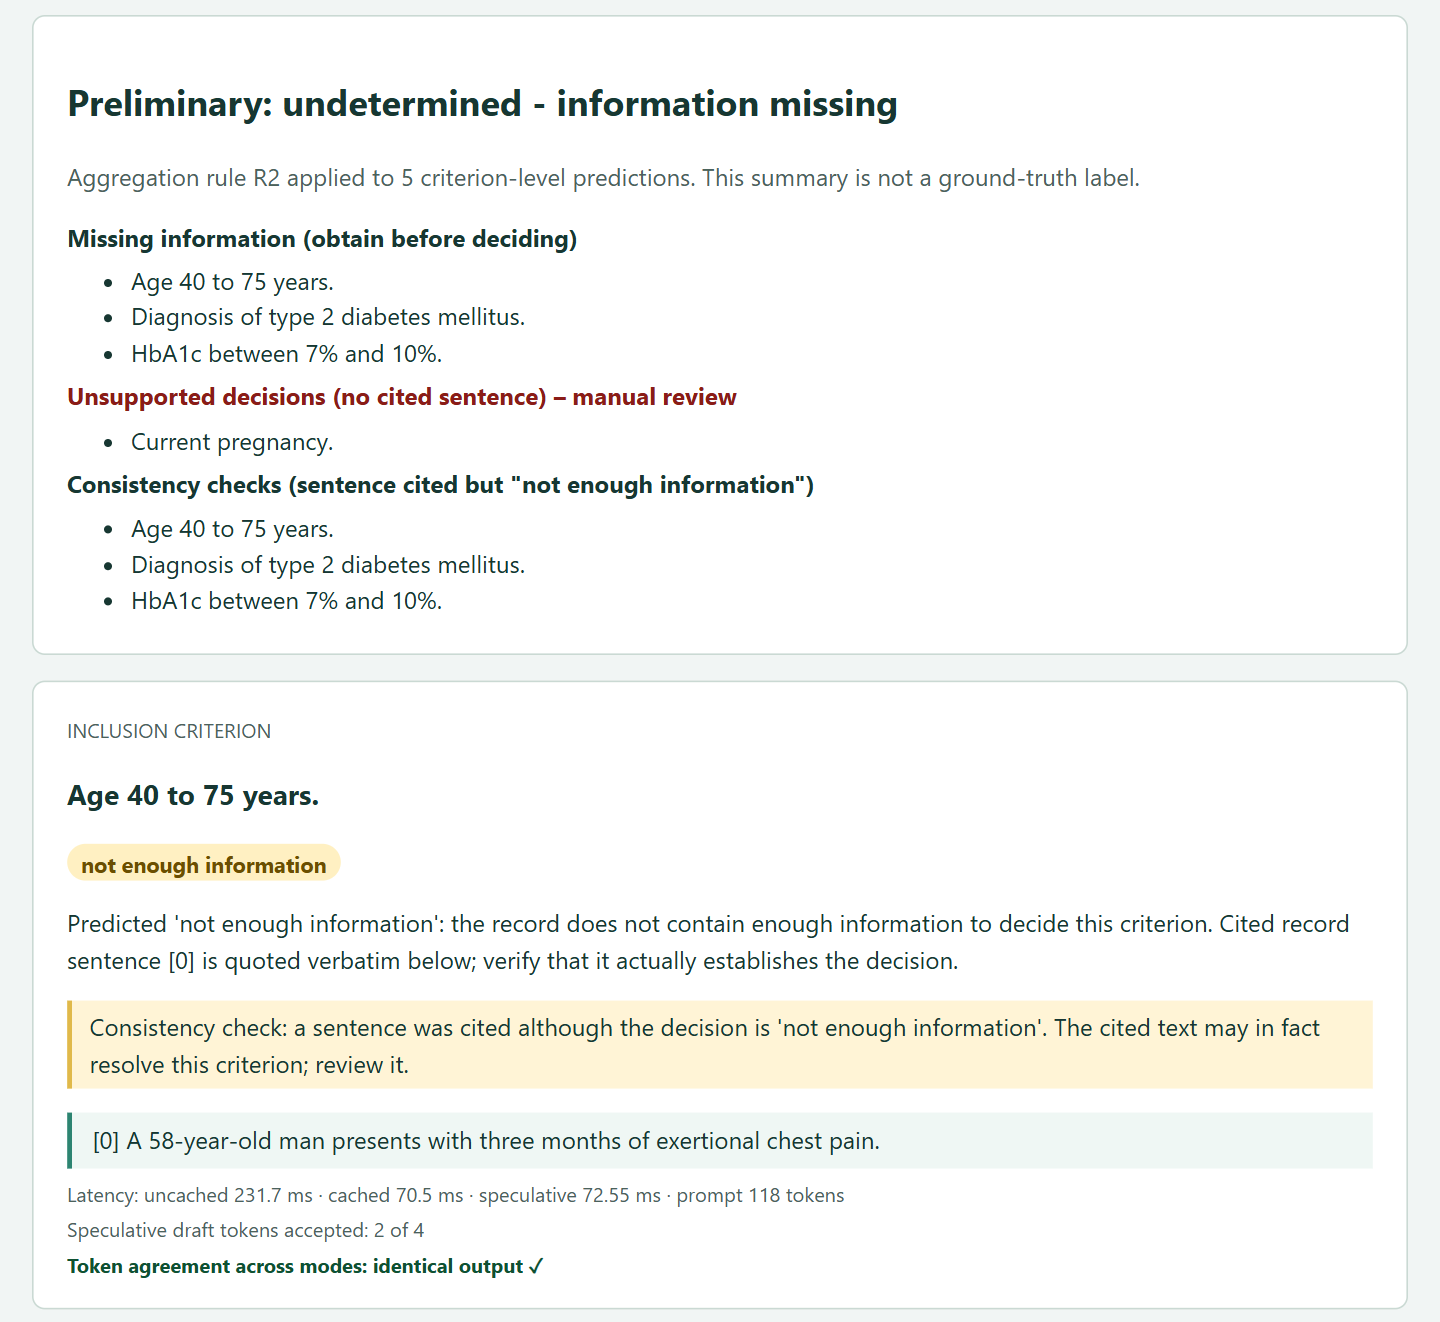
\includegraphics[width=0.485\textwidth]{application.png}\hfill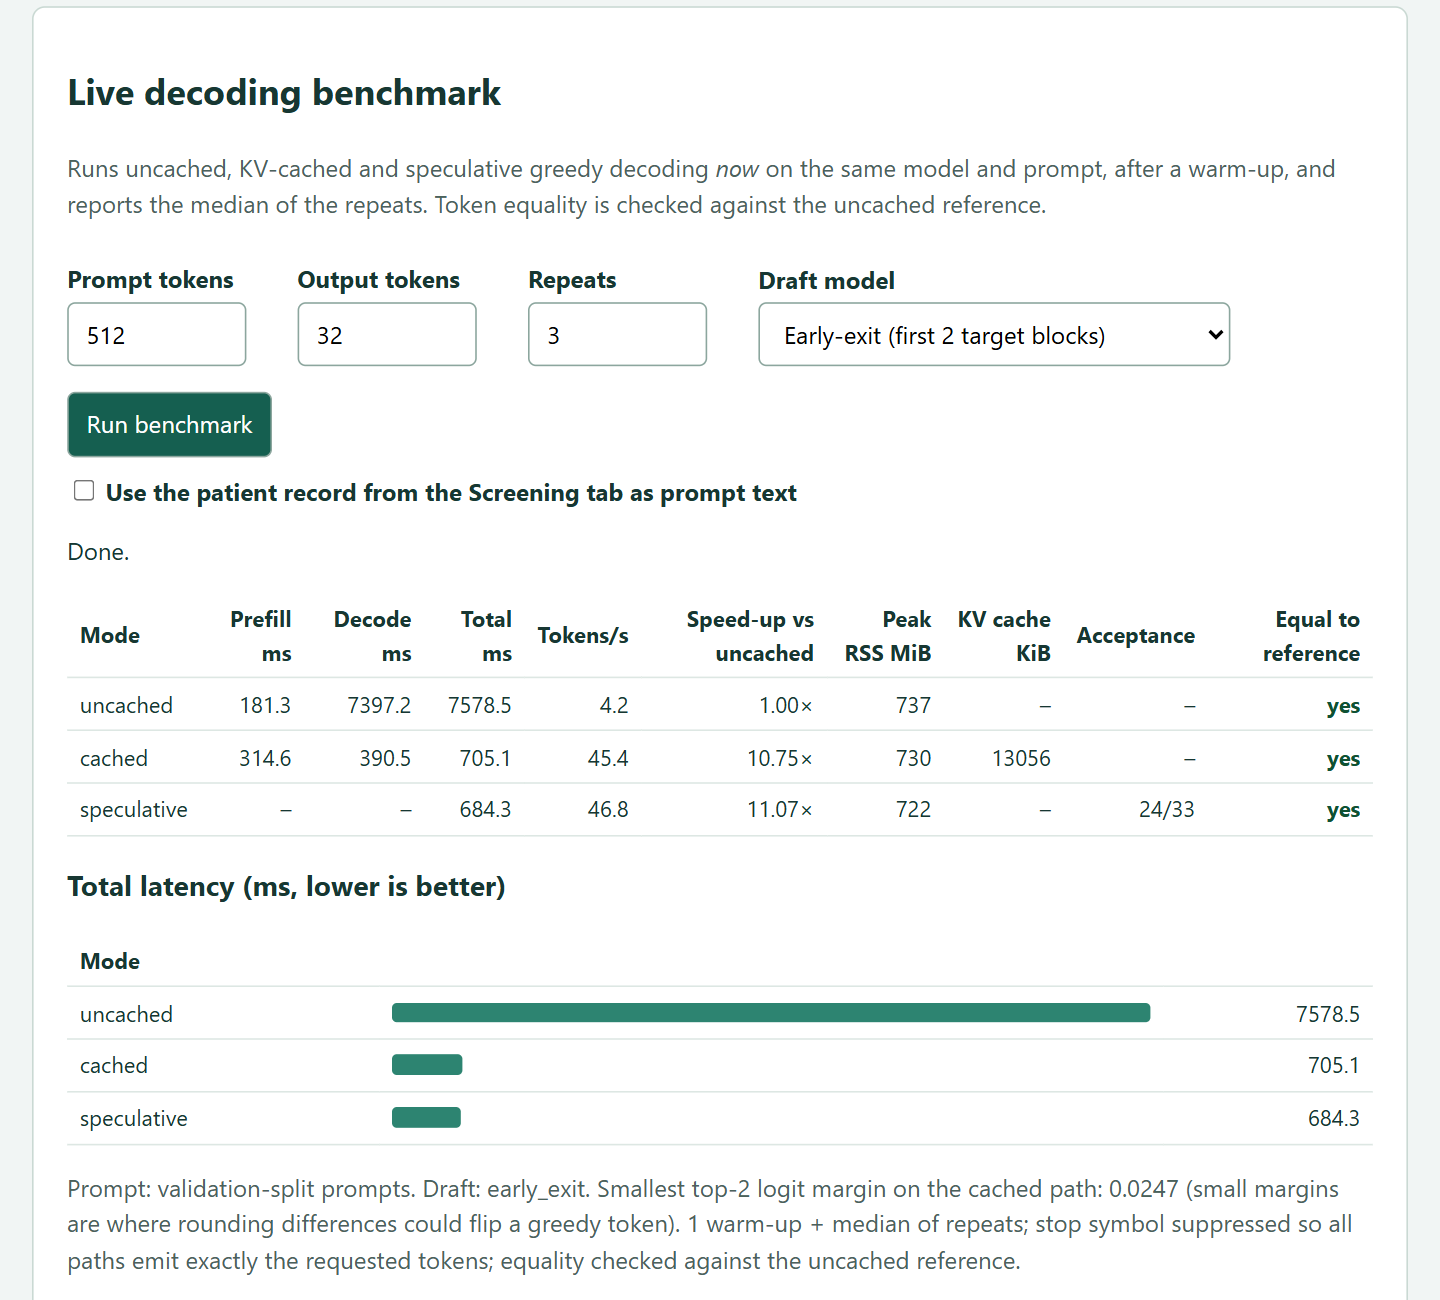
\includegraphics[width=0.485\textwidth]{lab.png}
\caption{Left: screening view (final model, compare mode, built-in example) with the applied rule, missing-information, unsupported and consistency-check lists, and a criterion card with verbatim evidence, per-mode latency, draft acceptance and token agreement. It shows the inclusion-side failure discussed in the text: the age sentence is cited, yet the label is NEI, and rule R5 flags it. Right: Inference lab, a fresh warmed benchmark at 512/32 tokens (median of 3) on the same model, with token equality for all three paths.}\label{fig:app}\end{figure*}

\subsection{KV caching}
Table~\ref{tab:runtime} reports the controlled decoding benchmark. In all 12 configurations every path produced exactly the uncached reference tokens (\texttt{verify.py} additionally checks 16 prompts). Prefill times are nearly equal between paths, as expected, because both process the full prompt once. The difference lies in decoding: the uncached path re-encodes $t$ tokens at step $t$, so its decode cost grows quadratically, while the cached path processes one token against a growing cache. The cached speed-up therefore grows with context: \CacheS$\times$ at 32/8, \CacheM$\times$ at 256/32 and \CacheL$\times$ at 1{,}024/64 tokens. The analytic KV cache is only 24\,KiB per token (26\,MiB at 1{,}088 positions), small next to the $\approx$650--810\,MiB process RSS dominated by the interpreter, PyTorch and both models' weights. Measured RSS differences between paths are within sampling noise; on a GPU or with long contexts and batching, cache memory, not compute, becomes the constraint~\cite{paged}. Cached and full-prefix logits differ by at most $7.3\times10^{-4}$ (chunk test). The smallest top-2 margin observed during cached decoding was \MinMargin{}, about 20$\times$ larger than that discrepancy, so no greedy flip occurred. Tighter margins could in principle flip a token, which is why the test compares tokens rather than assuming equivalence.

\subsection{Tiled attention}
Table~\ref{tab:attention} shows that both kernels match an FP64 ground truth on square, rectangular (cached-decoding), causal and non-causal shapes and on block sizes 8--128. The maximum absolute error is \AttnMaxErr{} (reference \AttnRefMaxErr), i.e.\ FP32 rounding. With logits of magnitude 7{,}200 a naive exponential overflows, while both max-shifted kernels stay finite and agree to $6\times10^{-8}$. The tiled kernel stores at most one $B\times B$ score tile (16\,KiB at $B{=}32$ versus 4\,MiB for the full 512$\times$512 matrix), but it is a median \TiledSlow$\times$ slower than the reference, which is itself \SdpaFast$\times$ slower than PyTorch's fused SDPA. Python loops dispatch many small matrix products, each with fixed overhead and poor cache reuse, whereas fused kernels keep tiles in registers/SRAM and avoid materialising intermediates~\cite{flash,flash2}. At these lengths the full score matrix fits in CPU cache anyway, so the memory saving cannot translate into speed; process RSS does not resolve such small buffers. Larger blocks reduce dispatch overhead: at 256$\times$256 the tiled kernel takes 74.7\,ms with $B{=}8$ but 1.40\,ms with $B{=}128$, close to the reference's 1.27\,ms. Causal tiling is cheaper than non-causal tiling (7.4 vs.\ 10.1\,ms at 256, 25.1 vs.\ 36.2\,ms at 512) because wholly-future tiles are skipped, the same saving that FlashAttention exploits.

\subsection{Speculative decoding}
Speculation produced the target's exact tokens in every benchmark and test, including forced all-accept, all-reject, mid-block stop and budget-limited paths and widths 1--8. In the logged benchmarks it never beat cached greedy decoding on this CPU (Tables~\ref{tab:runtime} and \ref{tab:screening}); in one live Inference-lab run at 512/32 tokens the early-exit draft was marginally faster (684 vs.\ 705\,ms at 73\% acceptance, Fig.~\ref{fig:app}), a difference within run-to-run noise. The early-exit draft reached speed-ups versus cached greedy of \SpecEES, \SpecEEM{} and \SpecEEL{} with acceptance \AccEES, \AccEEM{} and \AccEEL. The distilled 14M draft reached \SpecSmS, \SpecSmM{} and \SpecSmL{} with acceptance \AccSmS, \AccSmM{} and \AccSmL. Two measurements explain this. First, \emph{draft cost}: at batch size 1 on CPU a single-token step costs 6.27\,ms for the target, 2.15\,ms for the early-exit draft and 2.88\,ms for the 14M draft. Drafts are only 2--3$\times$ cheaper because per-call overhead, not FLOPs, dominates small models. With cost ratio $c\approx0.35$--0.46 and $k{=}4$, speculation needs acceptance well above 60--70\% before a round of four draft steps plus one verification beats four target steps. Second, \emph{distribution shift}: the 14M draft was distilled on real screening answers, where it agrees 96\% of the time (55/57; Table~\ref{tab:screening}), but the controlled benchmark forces long sequences over a fixed symbol alphabet that the target never produces in practice, and there acceptance falls to 6--7\%. The early-exit draft shares the target's lower layers and generalises better to those artificial sequences (55--61\%). On real screening outputs (2.33 symbols on average) the 14M draft's high acceptance still loses to cached greedy (106.0 vs.\ 88.4\,ms per criterion), because a second model's prefill and an extra verification pass cannot be amortised over two or three tokens. Speculation pays off for long outputs, with expensive targets, and on hardware where verifying $k$ tokens costs about as much as generating one (GPUs). Our measurements show where those conditions fail.

\subsection{Browser application}
Fig.~\ref{fig:app} shows the screening view after a comparison run and the Inference lab. All three decoding modes agree on every criterion; latencies and draft acceptance are measured on the user's own request, and the Inference lab reproduces the controlled benchmark live for any prompt length up to 1{,}024 tokens. During testing the application rejected 14 malformed requests with specific messages (e.g.\ duplicate sentence IDs, criteria without a type, oversize prompts, non-JSON bodies) and recovered without restarting. We also found and fixed a deployment bug: Python's default \texttt{SO\_REUSEADDR} on Windows let a second server bind the same port silently, so the launcher could talk to a stale instance. The server now binds exclusively and detects an existing instance through \texttt{/health}.

